\section{Motivation}
\label{sec:motivation}
As mentioned in section \ref{sec:intro}, the pros and cons are list in the follwing table \ref{table:regVsirreg}. Regular prefetchers are good at prefetching regular patterns while prefetching irregular patterns inaccurately. on the other hand, irregular prefetchers are good at prefetching irregular patterns while prefetching regular patterns inefficiently. Obviously, the advantage and disadvantage of these two kinds of prefetchers are complimentary. One straightforward idea is to identify regular patterns and irregular patterns during execution and apply corresponding prefetcher to issue prefetches.

\begin{table}[ht!]
\centering
\begin{tabular}{cccll}
\cline{1-3}
\multicolumn{1}{|c|}{}                     & \multicolumn{1}{c|}{Regular Access Pattern}             & \multicolumn{1}{c|}{Irregular Access Pattern}          &  &  \\ \cline{1-3}
\multicolumn{1}{|c|}{Regular Prefetcher}   & \multicolumn{1}{c|}{Accurate}              & \multicolumn{1}{c|}{{\color[HTML]{FE0000} Inaccurate}} &  &  \\ \cline{1-3}
\multicolumn{1}{|c|}{Irregular Prefetcher} & \multicolumn{1}{c|}{{\color[HTML]{FE0000} Inefficient}} & \multicolumn{1}{c|}{Accurate} &  &  \\ \cline{1-3}
\end{tabular}
\caption{Regular Vs. Irregular}
\label{table:regVsirreg}
\end{table}

  \subsection{Irregular Vs. Regular}
  \label{sec:irrVsre}
  Here we will show the performance graph of one regular benchmark and one irregular benchmark. In Fig.\ref{fig:regVsirreg}, \emph{libquantum} is a regular benchmark while \emph{omnetpp} is sort an irregular benchmark. We can see that, though \emph{ISB} and \emph{BO} have similar accuracy but \emph{BO}'s coverage is better, result in much more speedup than \emph{ISB}'s. That's why we call irregualr prefetchers are inefficient in detecting regular patterns. On the other hand, \emph{ISB} is much better than BO for benchmark \emph{omnetpp}. \emph{BO} even causes negative coverage because of huge cache pollution. This example shows that choosing right prefetcher for one kind of access pattern is crucial to improve benchmark performance.
  \begin{figure}[ht!]
	  \centering
	  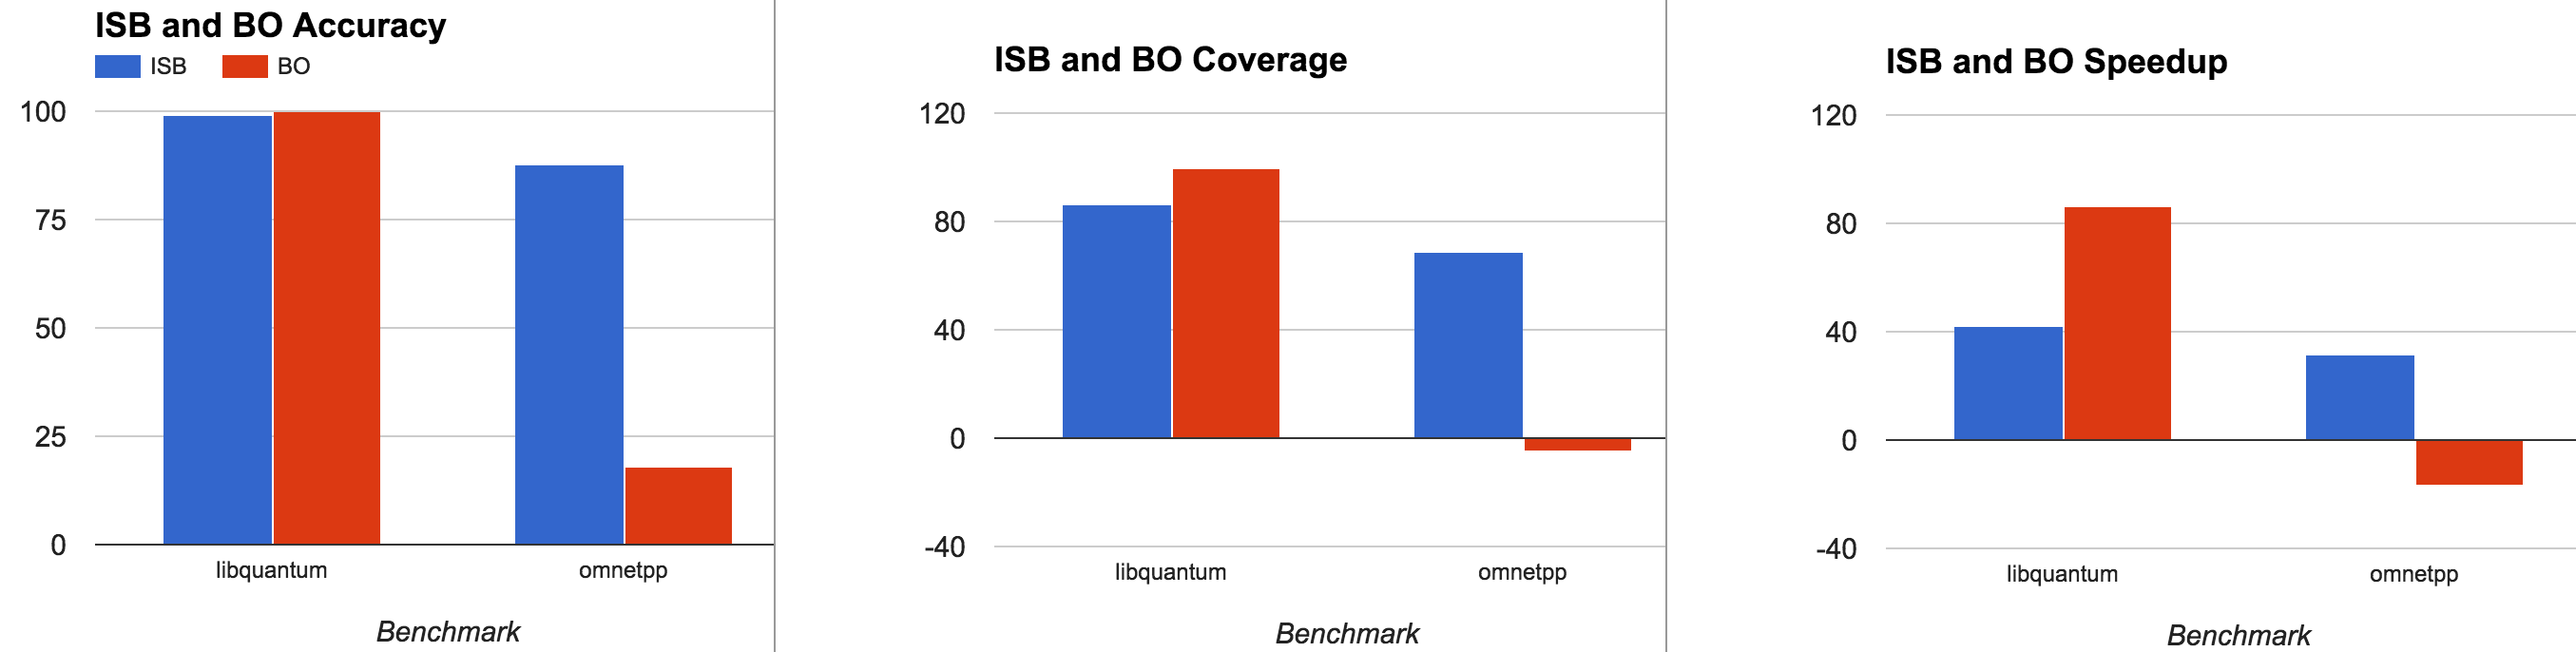
\includegraphics[width=1.0\textwidth]{images/isbvsbo.png}
	  \caption{\emph{ISB} and \emph{BO} performance comparision}
	  \label{fig:regVsirreg}
  \end{figure}


  \subsection{Naive Hybrid Prefetcher Vs. \emph{BO}\&\emph{ISB}}
  \label{sec:naivehy}
  One may ask a question after reading \ref{sec:irrVsre}: then why not issuing prefetches from both prefetchers? We call hybrid prefetcher with this behavior as \emph{naive hybrid prefetcher, or NHP}.
  \begin{figure}[ht!]
	  \centering
	  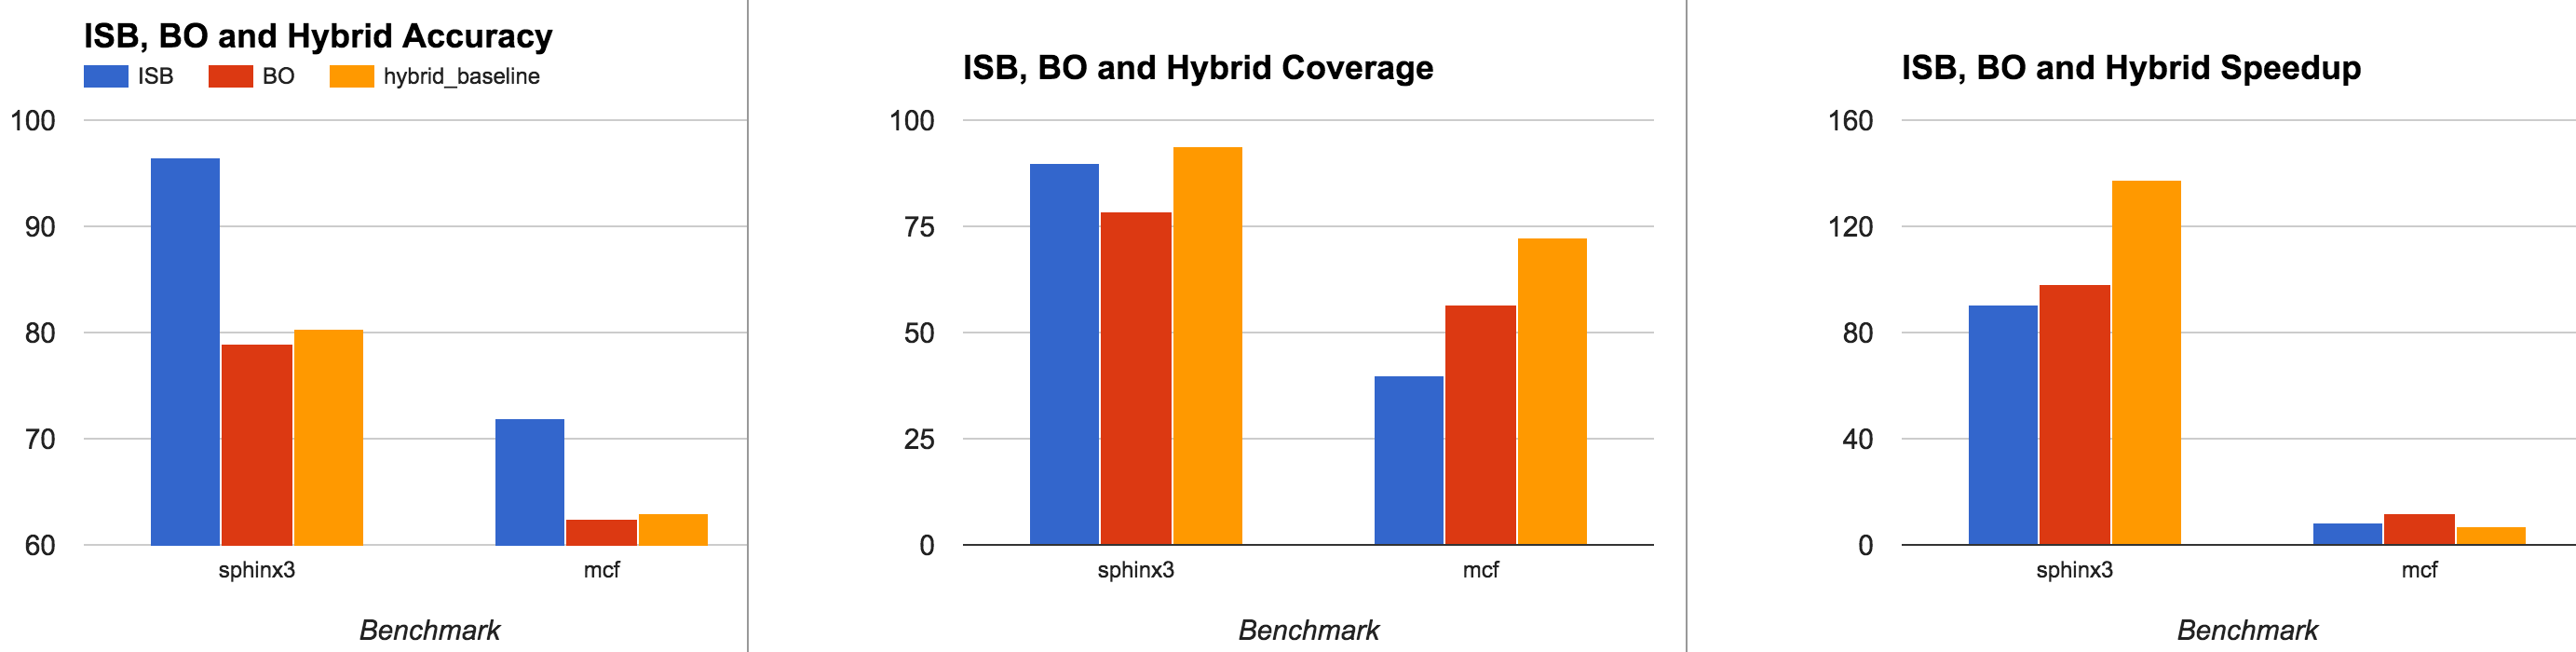
\includegraphics[width=1.0\textwidth]{images/hybridVssingle.png}
	  \caption{\emph{Naive Hybrid} and \emph{ISB, BO} performance comparision}
	  \label{fig:hybridVssingle}
  \end{figure}

  Well, it works when resource is enough rich, such as huge cache, huge memory bandwidth and so on. If these are limited, \emph{NHP} may cause huge memory pressure and cache pollution due to large number of inaccurate prefetches. In Fig.\ref{fig:hybridVssingle}, we give an example when \emph{NHP} works and when it doesn't. For benchmark \emph{sophinx3}, it is not memory intensive. The figure shows that the accuracy of \emph{ISB} is much higher than \emph{NHP}'s while \emph{NHP}'s coverage is much higher. It means that \emph{NHP} issued much more useless prefetchers to the cache. However, \emph{NHP}'s speed is still much better than \emph{ISB}'s. On the other hand, for benchmark \emph{mcf}, \emph{ISB} still has higher accuracy and lower coverage. However, this time, \emph{NHP}'s speed up is lower than \emph{ISB}'s. The possible reasons that a \emph{NHP} results in poor performance are listed below.

  \begin{itemize}
    \item Memory bandwidth is limited
    \item Memory request buffer size is limited
    \item Cache size is limited
    \item Cache pollution
  \end{itemize}

  \subsection{Previous Solution}
  \label{sec:PrevSol}
  previous solution

\subsection{Our Goal}
  \label{sec:goal}
  Our design of hybrid prefetcher should do prefetches smartly. Idealy, if our hybrid prefetcher can utilize \emph{BO} and \emph{ISB}'s advantage well while avoiding the influence of their disadvantages, the hybrid prefetcher should enjoy better accuracy, coverage and speedup. 
